\documentclass{beamer}
%
%\setbeameroption{show only notes}
%\setbeameroption{show notes}
%
% Choose how your presentation looks.
%
% For more themes, color themes and font themes, see:
% http://deic.uab.es/~iblanes/beamer_gallery/index_by_theme.html
%
%\mode<presentation>
%{
%  \usetheme{default}      % or try Darmstadt, Madrid, Warsaw, ...
%  \usecolortheme{default} % or try albatross, beaver, crane, ...
%  \usefonttheme{default}  % or try serif, structurebold, ...
%  \setbeamertemplate{navigation symbols}{}
  \setbeamertemplate{caption}[numbered]
%}

\mode<presentation>{}
\usepackage{beamerthemesplit}
\usepackage{animate}
\setbeamertemplate{footline}[frame number]
\setbeamertemplate{headline}{}
\setbeamertemplate{blocks}[rounded][shadow]
\setbeamercolor{block body}{bg=structure!10}
\setbeamercolor{block title}{bg=structure!20}
\usepackage[T1]{fontenc}
\usepackage[utf8]{inputenc}
 
\graphicspath{{../Logos/}}


\title[Title]{Your title is here}
\author{Xxxxxx XXXXXX}
\author{Xxxxxx XXXXXX}

\institute[CNRS / AMU]{Institut de Neurosciences de la Timone\\ CNRS and Aix-Marseille Université, France}
\date{}

%%% BIBLIO
\usepackage[backend=biber,
url=false,
doi=true,
isbn=false,
eprint=false,
style=nature,natbib=true]{biblatex}
\addbibresource{XXXXX.bib}


\usepackage{pgfgantt}
\usetikzlibrary{positioning}
\usetikzlibrary{backgrounds}
\definecolor{Maroon}{cmyk}{0, 0.87, 0.68, 0.32}
\definecolor{RoyalBlue}{cmyk}{1, 0.50, 0, 0}
\definecolor{OliveGreen}{rgb}{0,0.6,0}
\definecolor{Black}{cmyk}{0, 0, 0, 0}
\setganttlinklabel{f-s}{}%{FINISH-TO-START}
 \pgfkeys{
   /pgfgantt/ganttgroup inline label node/.style={
       shape=rectangle, draw=black, fill=white, anchor=north
       }
 }

\begin{document}

%\begin{frame}
%  \titlepage
 
%\end{frame}

\begin{frame}{First slide title}

\begin{figure}[p]
\centerline{
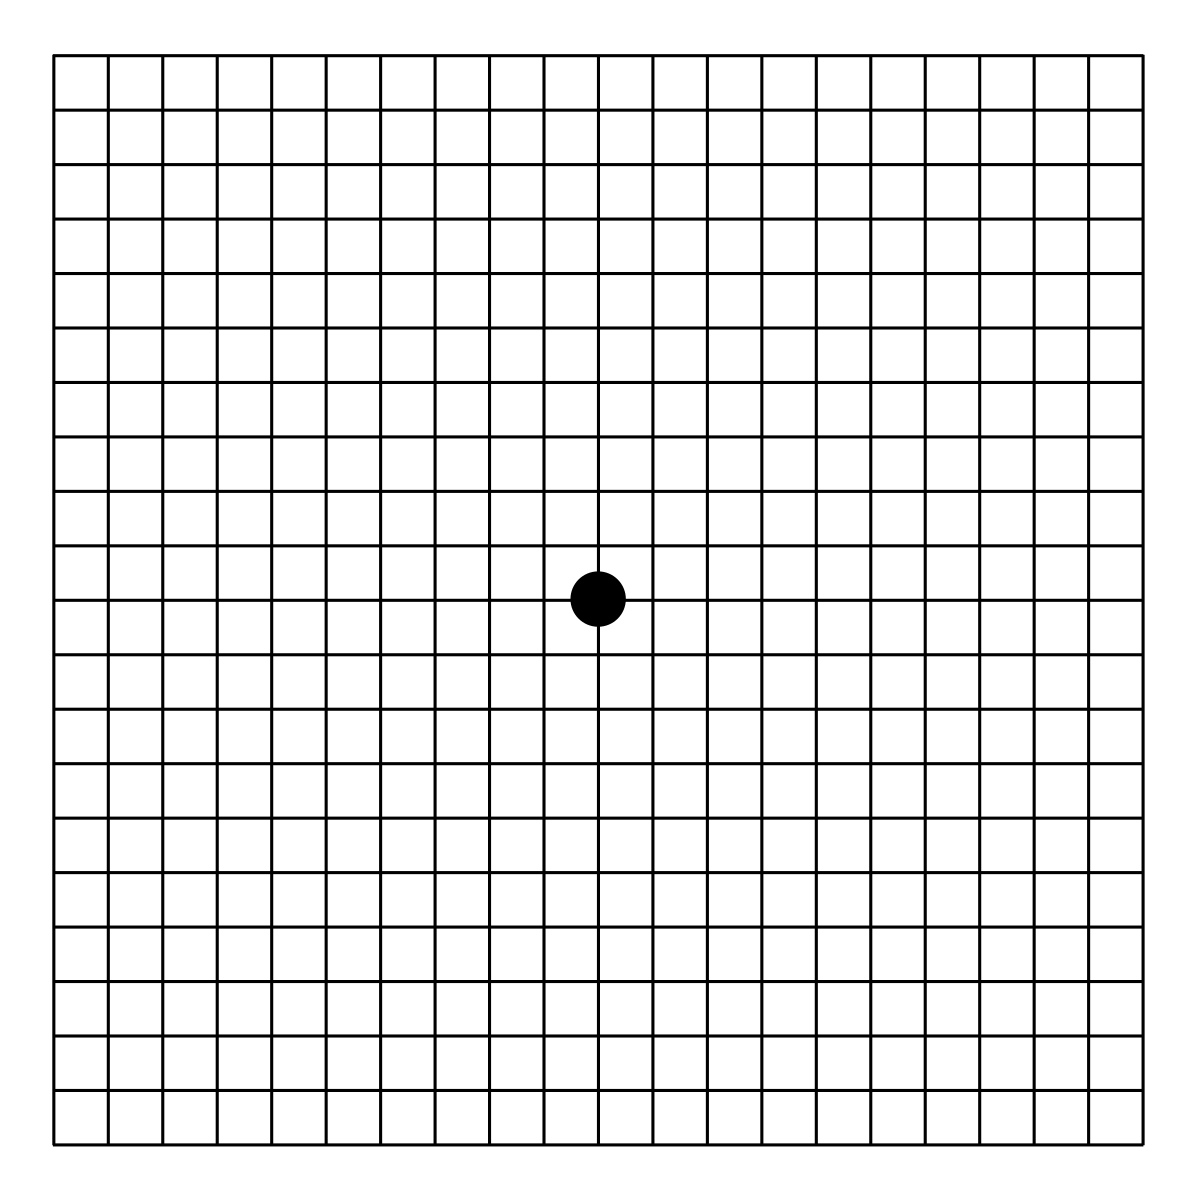
\includegraphics[width=.5\linewidth]{Logos/grid_display.png}}
\label{fig:1}
\end{figure}

\end{frame}

% Uncomment these lines for an automatically generated outline.
%\begin{frame}{Outline}
%  \tableofcontents
%\end{frame}

\section{Introduction}

%\begin{frame}{Plan}

%\begin{itemize}
%  \item 0'- 1' Introduction : Presentation of the different tools and notions
%  \item 1'- 2' DCNN limites : Robusteness + calcul cost 
%  \item 2'- 5' Human performances : Retinotopy
%  \item 5'- 10' Using Retinotopy to improve Computer vision, log polar referential
%  \item 10'- 13' Results and improvement 
%  \item 13'- 15' Opening and applications -> Neurosciences and Computational : Neurocomputational field
%\end{itemize}%

%\end{frame}
\begin{frame}{Deep Learning, useful tools for sciences}

\begin{figure}[p]
\begin{block}{To add different object}
\end{block}
\centerline{
\includegraphics<2->[width=.5\linewidth]{Logos/grid_display.png}
\includegraphics<3>[width=.5\linewidth]{Logos/grid_display.png}}
\label{fig:2}
\end{figure}

\end{frame}


\begin{frame}{Conclusion}
\begin{block}{Take away message:}
- Xxxxxxxxxxxxxxxxxxxxxxxxxxxxxxxxxxxxxxxxxxxxxxxxxxxxx \\
- Xxxxxxxxxxxxxxxxxxxxxxxxxxxxxxxxxxxxxxxxxxxxxxxxxxxxx \\

\end{block}
\begin{figure}[p]
\centerline{
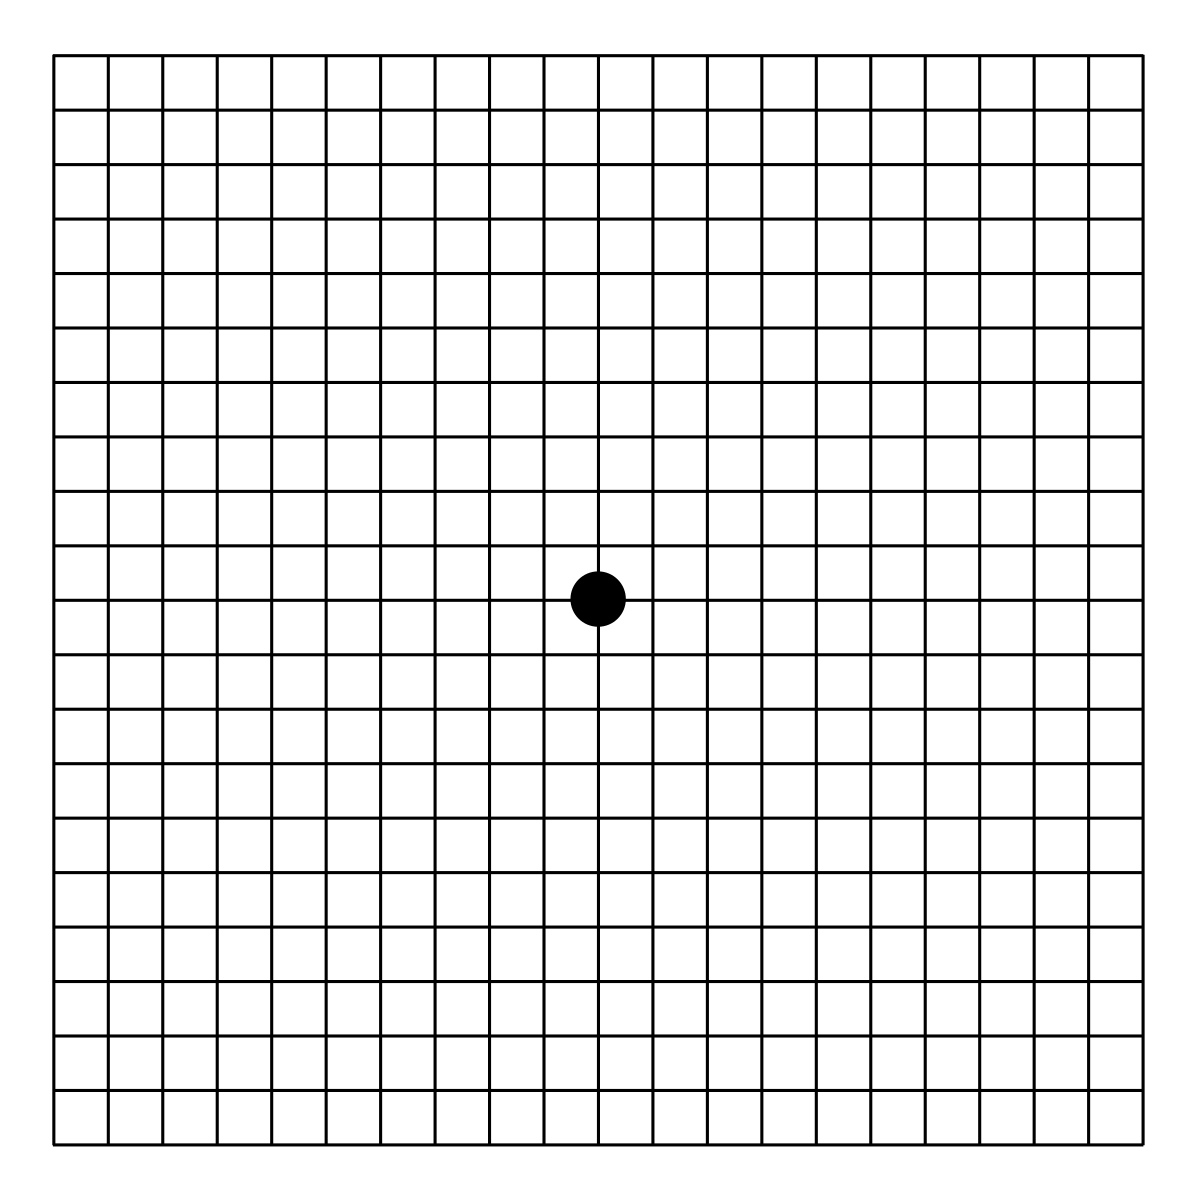
\includegraphics[width=.35\linewidth]{Logos/grid_display.png}}
\label{fig:qr}
%\url{https://laurentperrinet.github.io/grant/anr-anr/}
\end{figure}
\note{
    \begin{itemize}
            \item ... bla bla bla 

        \item bla bla bla 

%  07'  28''

    \end{itemize}}

\end{frame}


\end{document}



